\documentclass[11pt,a4paper]{report}

\usepackage[T1]{fontenc}
\usepackage[utf8]{inputenc}
\usepackage{lmodern}
\usepackage[margin=2.6cm]{geometry}
\usepackage{amsmath,amssymb}
\usepackage{booktabs}
\usepackage{tabularx}
\usepackage{longtable}
\usepackage{array}
\usepackage{xcolor}
\usepackage{tikz}
\usetikzlibrary{positioning,arrows.meta,fit,backgrounds,calc,shapes.multipart}
\usepackage[hyphens]{url}
\usepackage[hidelinks]{hyperref}
\usepackage[numbers,sort&compress]{natbib}
\usepackage{caption}
\captionsetup{font=small,labelfont=bf}

% A source reference: repository-relative path and line, set verbatim.
\makeatletter\g@addto@macro\UrlBreaks{\do\_}\makeatother
\newcommand{\src}[1]{{\footnotesize\path{#1}}}
\newcommand{\ty}[1]{\texttt{#1}}
\newcommand{\D}{\textsf{D}}   % device
\newcommand{\Hh}{\textsf{H}}  % host
\emergencystretch=3em
\newcolumntype{Y}{>{\raggedright\arraybackslash}X}

\title{Multi-Typed Gene Expression Programming on the GPU:\\[4pt]
\large The Master Symbol Table, the Geneframe, and a Device-Resident\\ Evolutionary Engine for Several Program Kingdoms}
\author{A report on the fuller and phylu systems designed by Andrew Morgan\\[2pt]
\small Gamakon Ltd.}
\date{1 November 2026\\[2pt]\small fuller \texttt{d450a10f} (branch \texttt{feat/futhark-kingdom}),
phylu \texttt{b79f3c38} (branch \texttt{feat/shape-typed-kingdom})}

\begin{document}
\maketitle

\begin{abstract}
This report describes, and checks against its source code, a multi-typed form of
gene expression programming (GEP) designed by Andrew Morgan and implemented in two
Rust systems: fuller, which owns the data model, and phylu, which owns the
evolutionary engine on the graphics processor (GPU). The design keeps
Ferreira's fixed-length Karva genotype but gives every gene a separate head and
tail for each output type. A slot that requires type $T$ reads the next unused
row of $T$'s reading frame, so every expressed node has the type its parent's
argument slot asks for, and every gene in every population expresses a feasible
program. There is no repair, rejection or fallback symbol: legality is a
property of the layout. Head lengths are derived from a declared program size,
$h_T=[T=R]+(N-1)\,a_T$, and the tail bound is exact per producer type. The
kingdom, that is, the language being evolved, is a query over a master symbol
table whose rows carry ordered, typed argument signatures; the population is a
table, the geneframe. The same typed core draws, varies, decodes and selects
the population in WGSL compute kernels on the device for four kingdoms:
symbolic regression (SR), POSIX-style regular expressions, WGSL compute kernels,
and Futhark array programs.

We establish, stage by stage and with file and line references, where each part
of the generation runs. For SR and regular expressions the whole generation
--- initialisation, expression, variation, program building, execution, fitness
evaluation by the hyperspherical fitness function, and selection --- runs on
the device, and the host reads back a frame of a few kilobytes. For the WGSL and
Futhark kingdoms the population, variation and selection are on the device, but
expression, program building (shader or compiler text, then a host compiler)
and fitness evaluation run on the host, and the fitness is written back to the
device for selection; one Futhark runner has no device population at all. We
report the measured results with their sources and limits, among them
non-regression of SR on 1,000 seed-runs, a held-out recall of 100.0\,\% on a
postcode task, a WGSL k-means centroid update at 0.0273 of the reference's
time (of which evolution contributed 1.6\,\%), a Futhark kernel that compiles
for the device where the reference does not, and a set of Futhark benchmarks on
which evolution did not find the target program.
\end{abstract}

\tableofcontents

%======================================================================
\chapter{Introduction}
\label{ch:intro}

Genetic programming (GP) searches a space of programs by variation and
selection~\cite{koza1992gp}. Two questions shape every GP system: how the
genotype is represented, and how the phenotype --- the program --- is kept
legal under variation. Gene expression programming
(GEP)~\cite{ferreira2001gep,ferreira2006book} answers the first with a fixed-length
linear genotype, the Karva gene, whose head and tail lengths guarantee that any
gene expresses a complete tree. It does not answer the second for typed
languages: classical GEP has one type, and a real programming language has
many.

This report describes a design that answers both together. Andrew Morgan's
design, developed in fuller and phylu over 2026, has three parts:
\begin{enumerate}
\item \textbf{The master symbol table and the geneframe.} Each symbol is a row
with an output type and an ordered list of argument types. A kingdom (the
language a population is written in) is a query over the table. A population
is a table of gene rows, the geneframe, keyed by chromosome, gene, domain,
domain type and position.
\item \textbf{Multi-typed GEP.} Every gene carries a head and a tail
\emph{for every output type} its root can reach. The types are columns of the
gene: a slot that requires $T$ reads the next row of $T$'s frame. Because a
symbol appears in a frame only where its output type is that frame's type, every
gene expresses a well-typed tree, and when the types carry the language's
legality rules, a feasible program.
\item \textbf{A device-resident engine.} The population lives on the GPU. The
same WGSL kernels initialise, vary, decode and select it for every kingdom; a
kingdom contributes its symbol table and its fitness evaluation.
\end{enumerate}
The objective Andrew set for the work is stated in fuller's goal document:
``A true multi-typed Gene Expression Programming kingdom for WGSL: every gene
expresses a legal GPU program, because the symbol table's types describe
exactly the legal programs'' (\src{fuller/docs/GOAL.md:3}).

\section{Contributions}
\label{sec:contrib}

The contributions of the design, as built, are these.
\begin{enumerate}
\item A multi-typed Karva layout with a head and a tail per output type, and
exact head and tail bounds derived from the kingdom's ordered signatures and a
declared program size (Chapter~\ref{ch:schema};
\src{fuller/src/kingdom_contract.rs:326}, \src{:371}). With one type it reduces
to Ferreira's layout byte for byte.
\item A relational data model: a master symbol table with typed, many-hot and
ordered signatures; a kingdom as a query over it; the geneframe as the table of
gene rows; and population-wide shared definitions as rows of the same table
(Chapter~\ref{ch:geneframe}).
\item A typed evolutionary core in WGSL that initialises, decodes, varies and
selects a population for any kingdom that passes the kingdom check, with a host
twin for every kernel and tests that the two agree (Chapter~\ref{ch:gpu}).
\item Four kingdoms on that core --- SR, regular expressions, WGSL kernels and
Futhark array programs --- each with its type system (Chapter~\ref{ch:kingdoms}).
\item An account, per kingdom and per stage, of what runs on the device and
what on the host, with the reason for each host stage and what would move it
(Chapters~\ref{ch:exec} and~\ref{ch:evo}, Table~\ref{tab:where}).
\item The measured results, and the faults found while obtaining them
(Chapters~\ref{ch:eval} and~\ref{ch:discussion}).
\end{enumerate}

\section{This paper and its set}
This is the core paper of a set of five. It gives the shared material in full:
the schema, the master symbol table and the geneframe, the GPU implementation,
execution and fitness evaluation, and GPU-driven evolution. Four domain papers
follow it, one for each kingdom: symbolic regression with typed SR~\cite{tr_sr},
regular expressions~\cite{tr_regex}, Futhark~\cite{tr_futhark} and
WGSL~\cite{tr_wgsl}. Here each kingdom is given only its type system and its
place on the device.

\section{Method of this paper}
Every claim of where a stage runs was checked by reading the code at the
commits named on the title page; references take the form
\src{repository/path:line}. Every number is quoted from a measurement file in one
of the two repositories, named where it is used. Where a document and the code
disagree, the code is reported and the disagreement is noted. No new
experiment was run for this report.

\section{Terminology}
We use the vocabulary of evolutionary computation: an \emph{individual} (one
chromosome), its \emph{genotype} (the gene words) and \emph{phenotype} (the
expressed program), the \emph{population}, \emph{fitness evaluation},
\emph{selection}, \emph{mutation} and \emph{crossover}, \emph{constraints},
\emph{objectives}, and \emph{feasible} programs. The \emph{device} is the GPU;
the \emph{host} is the CPU process that drives it. A \emph{kingdom} is Andrew's
term for the language a population is written in.

%======================================================================
\chapter{Background}
\label{ch:background}

\section{Gene expression programming and the Karva notation}
In GEP~\cite{ferreira2001gep,ferreira2006book} a chromosome is one or more genes
of fixed length. A gene has a head of length $h$, which may hold functions and
terminals, and a tail of length $t=h(n-1)+1$, which holds terminals only, where
$n$ is the largest arity. The gene is read in level order (breadth first) from
its first position, the Karva notation: each function consumes the next
unread positions as its arguments. The tail length guarantees that the reading
never runs out of terminals, so every gene expresses a complete tree, and the
unread suffix is a non-coding region that variation can change without effect.
Genes of a multigenic chromosome are joined by a linking function, or by an
evolved homeotic gene~\cite{ferreira2006adf}; the latter makes the linker
itself subject to evolution, and Ferreira also gives automatically defined
functions (ADFs) in this form. Numerical constants are held in a separate Dc
domain indexed by a placeholder terminal (GEP-RNC)~\cite{ferreira2006book}.
GEP's operators are point mutation, inversion, IS, RIS and gene transposition,
and one-point, two-point and gene recombination.

The strength of the representation is that variation is cheap and closed: any
change to any position yields a gene that expresses. Its weakness, for typed
languages, is that classical GEP has one type.

\section{Typed and strongly typed GP}
Montana's strongly typed GP (STGP)~\cite{montana1995stgp} attaches a type to
every function argument and return value, and restricts initialisation and
crossover so that only well-typed trees are built. STGP keeps legality by
constraining each operator: crossover may only exchange subtrees of the same
type, and generation draws each child from the symbols of the required type.
Its genotype is the tree itself.

The design described here keeps STGP's type discipline and GEP's linear
genotype. The difference is where the constraint is enforced: in STGP each
operator is constrained; here the \emph{layout} is typed, so the unconstrained
operators of GEP --- applied within one type's domain --- cannot produce an
ill-typed child.

\section{Grammar-based GP and grammatical evolution}
Grammar-based GP~\cite{whigham1995grammar,mckay2010survey} uses a context-free
grammar to define the legal programs. Grammatical evolution
(GE)~\cite{ryan1998ge,oneill2001ge} uses a linear integer genotype whose codons
choose productions of a grammar, reading the codon modulo the number of
choices. GE's mapping is total, like GEP's, but the meaning of a codon depends
on everything read before it, so a change early in the genotype can rewrite the
whole phenotype (low locality). In the multi-typed layout a codon belongs to one
type's frame, and an edit in $\mathrm{head}_T$ changes only $T$'s bytes;
as in Karva it can change which rows of other frames are read, never their
types (\src{phylu/src/evolve/typed_vary.rs:1-20}; the locality tests of
\src{fuller/src/typed_gep_tests.rs}).

\section{GP on graphics processors}
Fitness evaluation dominates the cost of GP, and the GPU literature has largely
addressed it. Harding and Banzhaf~\cite{harding2007gpu} and
Chitty~\cite{chitty2007gpu} compiled or interpreted evolved expressions on
graphics hardware for data-parallel fitness evaluation. Langdon and
Banzhaf~\cite{langdon2008simd} ran a SIMD interpreter for linear GP on the GPU,
so that many individuals are evaluated by one kernel.
Robilliard, Marion-Poty and Fonlupt~\cite{robilliard2009gpu} interpreted a whole
population of tree programs on the device. Langdon's
overview~\cite{langdon2011overview} surveys this work: most systems keep
initialisation, variation and selection on the host and move evaluation to the
device. Augusto and Barbosa~\cite{augusto2013opencl} evaluate trees in parallel
with OpenCL, and TensorGP~\cite{baeta2021tensorgp} expresses the evaluation as
tensor operations. A separate line of work evolves GPU programs themselves:
Langdon and colleagues improved existing CUDA code by genetic
improvement~\cite{langdon2015cuda}, and superoptimisers such as
STOKE~\cite{schkufza2013stoke} and Souper~\cite{sasnauskas2017souper} search for
cheaper equivalents of given code.

This design differs from that literature in two ways. The population, its
variation and its selection run on the device as well as the evaluation, for
any kingdom; and for two of its kingdoms the phenotype is itself a GPU program
(a WGSL kernel or a Futhark program), so the device both evolves programs and
runs them.

\section{Equality saturation}
fuller uses equality saturation~\cite{tate2009equality} through
egglog~\cite{zhang2023egglog}, the successor of egg~\cite{willsey2021egg}, to
rewrite expressed programs into equivalent forms. In this report the e-graph
appears as a source of variation (rewritten individuals enter the population),
not as part of the typed core.

\section{The hyperspherical fitness function}
Selection reads one scalar. Where a kingdom has several objectives, they are
combined by Andrew's hyperspherical fitness function (HFF)~\cite{morgan2026hff}.
With $m$ objectives scaled to $x_i\in[0,1]$ (zero best), the TrueNorth form
lifts the point onto a sphere and returns its angle from the pole at the
origin; the energy score $e=1-\min(1,\sum_i x_i^2/m)$ is the cosine, so
\[
  \theta=\arccos e,\qquad 0\ \text{best},\ \pi/2\ \text{worst}
\]
(\src{hff/src/core_functions.rs:73}; device form \src{phylu/src/evolve/hff.wgsl:128}).

%======================================================================
\chapter{The Multi-Typed GEP Schema}
\label{ch:schema}

The schema was specified by Andrew in a design document (revision 4,
2026-10-20) and is implemented on the host in
\src{fuller/src/kingdom_contract.rs}, \src{fuller/src/typed_gep.rs} and
\src{fuller/src/typed_chromosome.rs}, and on the device in phylu's typed core.
The design document has since fallen behind the code in places; everything in
this chapter is stated from the code. Its objective is that every expressed
node has the type required by its parent's argument slot, for every gene and
every permitted variation, with no repair, substitution or fallback: ``a cell
that does not fit is a \texttt{LayoutDefect}, `our software has a bug: \ldots'\,''
(\src{fuller/src/typed_gep.rs:14-15}).

\section{The kingdom contract}
A kingdom is two relations (\src{fuller/src/kingdom_contract.rs:1-21}):
\begin{itemize}
\item $\mathit{symbol\_outputs}(\mathit{symbol},\mathit{output\_type})$, over
functions and terminals, with exactly one row per symbol; a polymorphic
spelling is one symbol per output type;
\item $\mathit{argument\_signature}(\mathit{symbol},\mathit{arg\_index},\mathit{required\_type})$,
keyed by symbol and argument index, so the order of a call's arguments is data.
\end{itemize}
The check \texttt{KingdomRelations::check} (\src{fuller/src/kingdom_contract.rs:84})
returns either a \texttt{KingdomContract} with the derived quantities below, or
every defect found, each reported as a bug in our software; a kingdom that fails
does not load. From the relations it derives
\begin{itemize}
\item $a_{T,U}$: the most arguments of type $T$ that any one function
outputting $U$ takes;
\item $a_T=\max_U a_{T,U}$ over the producers reachable from the root;
\item $n_U$: the largest arity among functions outputting $U$;
\item $\mathit{reachable}(R)$: the types reachable from a root $R$ through
signatures.
\end{itemize}

\section{Gene layout: a head and a tail for every type}
A gene rooted at $R$ has, for every reachable type $T$, a domain
$\mathrm{head}_T$, a domain $\mathrm{tail}_T$ and, for a type with a literal
domain, a $\mathrm{Dc}_T$ (Figure~\ref{fig:schema}). $\mathrm{head}_T$ holds
symbols whose output is $T$, functions or terminals; $\mathrm{tail}_T$ holds
terminals whose output is $T$; $\mathrm{Dc}_T$ holds indices into the constant
pool $C_T$. The physical order is every head, then every tail, then every Dc,
each in frame order with the root's type first, so that a one-type gene is
exactly Karva's head, tail and Dc (\src{fuller/src/typed_gep.rs:1-12}).

\paragraph{Head lengths from the program size.} A layout declares, for each
gene, its root type $R$ and a program size $N$, the number of expressed
functions the layout must hold. The head lengths are
\begin{equation}
  h_T=[T=R]+(N-1)\,a_T,\qquad T\in\mathit{reachable}(R),
  \label{eq:head}
\end{equation}
implemented in \texttt{heads\_from\_program\_size}
(\src{fuller/src/kingdom_contract.rs:326-333}). For the root type this is
$h_R=1+(N-1)\,a_R$. The bound is exact: in level order the last $T$ function
has before it at most the root and the $T$ slots opened by the other $N-1$
functions, at most $a_T$ each, and a chain of $N$ functions each giving its $T$
child last attains it. So every program of at most $N$ functions fits every
$\mathrm{head}_T$ whatever its type mix, and no type's head is a guessed budget.
The inverse, the largest $N$ a set of heads guarantees, is
\texttt{guaranteed\_program\_size} (\src{:338}).

\paragraph{The per-producer tail bound.} With heads fixed, the demand for $T$
is bounded by its producers and by the number of leaves
(\src{fuller/src/kingdom_contract.rs:366-391}):
\begin{align}
  P_T &= [T=R]+\textstyle\sum_U h_U\,a_{T,U}, &
  L   &= 1+\textstyle\sum_U h_U\,(n_U-1),\notag\\
  t_T &= \max\bigl(0,\ \min(P_T,\,L+h_T)-h_T\bigr), &
  d_T &= \min(P_T,\,L).
  \label{eq:tail}
\end{align}
With one type, $a_{R,R}=n_{\max}$, so $P=1+h\,n_{\max}$, $L=1+h(n_{\max}-1)$
and $t=d=h(n_{\max}-1)+1$: Ferreira's tail. The kingdom's test asserts this
(\src{fuller/src/kingdom_contract.rs:619-632}).

\begin{figure}[t]
\centering
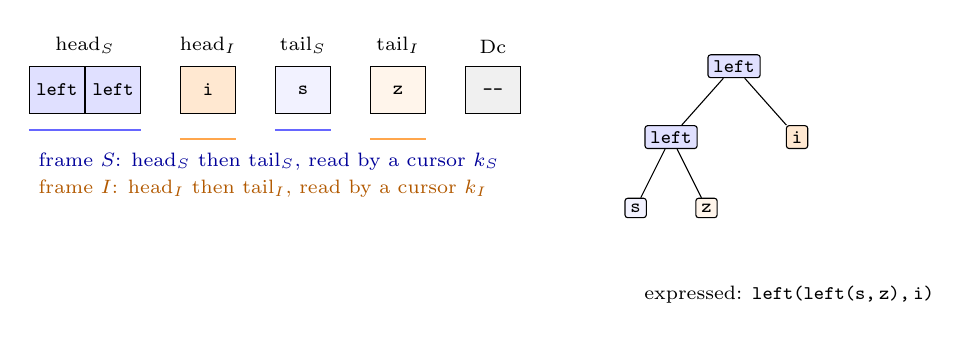
\begin{tikzpicture}[
  cell/.style={draw,minimum height=6mm,minimum width=7mm,font=\scriptsize\ttfamily,inner sep=1pt},
  lab/.style={font=\scriptsize},
  >=Stealth]
% one gene: head_S | head_I | tail_S | tail_I | Dc_I
\node[cell,fill=blue!12] (s0) at (0,0) {left};
\node[cell,fill=blue!12,right=0pt of s0] (s1) {left};
\node[cell,fill=orange!18,right=14pt of s1] (i0) {i};
\node[cell,fill=blue!5,right=14pt of i0] (ts0) {s};
\node[cell,fill=orange!8,right=14pt of ts0] (ti0) {z};
\node[cell,fill=gray!12,right=14pt of ti0] (dc0) {--};
\node[lab,above=1pt of s0.north east] {$\mathrm{head}_S$};
\node[lab,above=1pt of i0] {$\mathrm{head}_I$};
\node[lab,above=1pt of ts0] {$\mathrm{tail}_S$};
\node[lab,above=1pt of ti0] {$\mathrm{tail}_I$};
\node[lab,above=1pt of dc0] {Dc};
% frames
\draw[thick,blue!60] ([yshift=-2mm]s0.south west) -- ([yshift=-2mm]s1.south east);
\draw[thick,blue!60] ([yshift=-2mm]ts0.south west) -- ([yshift=-2mm]ts0.south east);
\draw[thick,orange!70] ([yshift=-3.2mm]i0.south west) -- ([yshift=-3.2mm]i0.south east);
\draw[thick,orange!70] ([yshift=-3.2mm]ti0.south west) -- ([yshift=-3.2mm]ti0.south east);
\node[lab,blue!60!black,anchor=west] at ([yshift=-6mm]s0.south west) {frame $S$: $\mathrm{head}_S$ then $\mathrm{tail}_S$, read by a cursor $k_S$};
\node[lab,orange!70!black,anchor=west] at ([yshift=-9.5mm]s0.south west) {frame $I$: $\mathrm{head}_I$ then $\mathrm{tail}_I$, read by a cursor $k_I$};
% tree
\begin{scope}[xshift=8.6cm,yshift=0.3cm,level distance=9mm,
  every node/.style={font=\scriptsize\ttfamily,draw,rounded corners=1pt,inner sep=2pt},
  level 1/.style={sibling distance=16mm},level 2/.style={sibling distance=9mm}]
\node[fill=blue!12] {left}
  child {node[fill=blue!12] {left} child {node[fill=blue!5] {s}} child {node[fill=orange!8] {z}}}
  child {node[fill=orange!18] {i}};
\end{scope}
\node[lab,align=center] at (9.3,-2.6) {expressed: \texttt{left(left(s,\,z),\,i)}};
\end{tikzpicture}
\caption{One gene of a two-type test kingdom:
\texttt{left}$:S(S,I)$, terminals \texttt{s}$:S$, \texttt{i}$:I$, and the polymorphic
spelling \texttt{z} as one symbol per type. Each argument slot asks for a type and
reads the next row of that type's frame, head first, then tail. The walk shown is
the one the test fixture asserts for $\mathrm{head}_S=(\texttt{left},\texttt{left})$,
$\mathrm{tail}_S=(\texttt{s})$, $\mathrm{tail}_I=(\texttt{z})$
(\protect\src{fuller/src/typed_gep_tests.rs:806-815}).}
\label{fig:schema}
\end{figure}

\section{Expression: the typed Karva walk}
Expression is deterministic (\src{fuller/src/typed_gep.rs:555-610}). A FIFO
queue starts with the root slot $(R,\text{depth }0)$ and a cursor $k_T=0$ for
each type. On dequeuing a slot of type $T$, the walk reads row $k_T$ of $T$'s
frame ($\mathrm{head}_T$ then $\mathrm{tail}_T$), increments $k_T$, and enqueues
the selected symbol's argument slots in signature order. An expressed constant
placeholder $?_T$ consumes the next $\mathrm{Dc}_T$ entry. The bounds of
equation~\eqref{eq:tail} guarantee that no frame runs out, and frame membership
proves the selected symbol has type $T$; a missing frame row is reported as a
defect in the kingdom or layout and is never repaired. The same walk and the
bound derivation are also written as recursive SQL over the geneframe's rows,
and a test runs them in
DuckDB on the fixtures and requires the host decoder to equal the query row for
row (\src{fuller/src/typed_gep_tests.rs:645-660}). The geneframe is, literally, a
table that can be expressed by a query.

\section{Variation: domains are invariant}
Every operator draws from a domain enumerated from the layout before the draw,
so every child is feasible by construction (host: \texttt{GeneLayout::alphabet},
\texttt{spans}, \texttt{Layout::homologous\_pairs}, \src{fuller/src/typed_gep.rs:181-330};
device: \src{phylu/src/evolve/typed_vary.rs:1-20}). Mutation in $\mathrm{head}_T$ draws any symbol outputting $T$; in
$\mathrm{tail}_T$ any terminal outputting $T$; in $\mathrm{Dc}_T$ any valid
index. Inversion, IS and RIS transposition stay inside one (gene, domain, type).
One-point, two-point and gene recombination exchange homologous coordinates only:
same layout, gene id, domain, type and local position. Gene transposition moves
a gene only between gene ids that the layout gives the same root type and the
same head lengths. An operator whose domain is empty for a layout is absent from
that layout's schedule, rather than drawn and replaced.

\paragraph{Write-back.} Every rewrite of an expressed tree --- the e-graph's
variants, constant snapping, folding, cleansing --- is encoded back into a gene
by the walk in reverse: the $k$-th $T$ node of the level order is placed at row
$k$ of $T$'s frame (\src{fuller/src/typed_gep.rs:688}). With $j_T$ one more than
the rank of the last $T$ function, a tree is encodable exactly when $j_T\le h_T$
for every $T$ (\texttt{required\_heads}, \src{:615}; \texttt{fits}, \src{:678}).
Removal-only rewrites never raise any $j_T$ and always fit. In phylu, every host
rewrite goes through this encoder (\texttt{GeneCodec},
\src{phylu/src/evolve/typed_write_back.rs}), and a rewrite that does not fit is a
named defect.

\section{Size of the layout}
The bounds make the gene width a consequence of the kingdom and $N$, not a
tuned buffer. Table~\ref{tab:bounds} gives the bounds for SR and for the base
regex relations, computed for this paper from equations~\eqref{eq:head}
and~\eqref{eq:tail} over the rows in \src{fuller/src/geneframe.rs:527-561} and
\src{fuller/src/kingdom_contract.rs:471-486}; the kingdom check prints the same
table for every kingdom (\texttt{the\_kingdom\_reports\_print},
\src{fuller/src/kingdom_contract.rs:807}). The regex rows show the per-producer
bound at work: \ty{Char} is demanded by \texttt{lit} and twice by each class
range, so $P_{\mathrm{Char}}=15+2\cdot14=43$, but at most $L=30$ leaves exist, so
$t_{\mathrm{Char}}=\min(43,30+14)-14=29$. The WGSL kingdoms, with hundreds of
types, need genes wider by orders of magnitude; the geneframe is therefore
allocated in full and paged across device buffers, never bounded to fit one.

\begin{table}[t]
\centering\small
\caption{Bound table for a gene of program size $N$, computed from the kingdom
contract's formulas (\protect\src{fuller/src/kingdom_contract.rs:326-391}) over
the committed rows. Width is $\sum_T(h_T+t_T)+\sum_{T\ \mathrm{constant}}d_T$
32-bit words.}
\label{tab:bounds}
\begin{tabular}{@{}lrrrrl@{}}
\toprule
kingdom & $N$ & types & $L$ & width & per type ($h,P,t,d$)\\
\midrule
SR    & 8  & 1 & 16 & 47  & \ty{F}: 15, 31, 16, 16\\
SR    & 32 & 1 & 64 & 191 & \ty{F}: 63, 127, 64, 64\\
regex & 8  & 4 & 30 & 177 & \ty{Pattern} 15, 31, 16, --; \ty{CharClass} 14, 43, 29, --;\\
      &    &   &    &     & \ty{Char} 14, 43, 29, 30; \ty{I} 7, 15, 8, 15\\
\bottomrule
\end{tabular}
\end{table}

\section{Constants}
A constant-capable type $T$ has a placeholder terminal $?_T$ and a domain
$\mathrm{Dc}_T$ of length $d_T$. Only an expressed placeholder consumes the next
entry. The pool $C_T$ is append-only for a population epoch, so an index once
written stays valid. Dc variation stays in its own $(\text{gene},T,\text{Dc})$
domain.

\section{The head draw}
The layout does not say how often a head cell holds a function. The
initialiser and head point mutation, on host and device, read a
\texttt{FunctionShare} per type: \texttt{Proportional} (Ferreira's practice, a
head symbol drawn from the whole set of the cell's type), \texttt{Half} (a fair
coin per cell) or \texttt{Fixed(p)}, and optionally force the root cell to a
function (\src{phylu/src/evolve/typed_init.rs:21-56}). Which draw searches best
has not been settled by a measurement.

%======================================================================
\chapter{The Master Symbol Table and the Geneframe}
\label{ch:geneframe}

The data model is Andrew's, adopted into fuller and owned there
(\src{fuller/src/geneframe.rs:1-28}). Its founding observation is that a Karva
chromosome, rotated through ninety degrees and stacked with the others of its
population, is a table: position becomes a column value, and the population can
be queried, exchanged and stored as rows.

\section{The master symbol table}
The master symbol table holds every symbol of every kingdom
(\texttt{SymbolTable}, \src{fuller/src/geneframe.rs:302}). A row carries a kingdom,
a symbol number (positive for a function, negative for a terminal), a semantic
id that fuller rewrites on, a target-language spelling, and a typed
\emph{many-hot} arity: a count of inputs and outputs per type
(\texttt{Arity}, \src{:260-283}). A function such as
\texttt{acquire} with two \ty{ORG} arguments, one \ty{MONEY} and one \ty{NP} has
four non-zero input columns; the integer arity of classical GEP is their sum.

The type set is declared once (\texttt{Ty}, \src{fuller/src/geneframe.rs:46-127}):
base types (\ty{S}, \ty{I}, \ty{F}, \ty{B}, \ty{A}, \ty{L}); the transcendental
depth types \ty{T1} and \ty{T2}; NLP and regex types; and four table-defined
families --- \ty{Wgsl(u16)}, \ty{Tsr(u16)}, \ty{Futhark(u16)} and
\ty{Futhark(u16)} --- whose members are rows of a generated
\texttt{types.tsv}, so that a new type in those kingdoms is a table row, not a
code change. A type has a device code (\texttt{Ty::code}, \src{:168}).

The many-hot arity is keyed by type and so cannot hold argument order
(\texttt{regex\_rep\_n} takes \ty{(Pattern, I)}, which a type-keyed map reads
back as \ty{(I, Pattern)}). The kingdom contract's ordered
$\mathit{argument\_signature}$ relation carries the order
(\src{fuller/src/geneframe.rs:518-527}, \src{fuller/src/kingdom_contract.rs:8-10}).

\section{A kingdom is a query}
A kingdom is a filter over the master table (\texttt{SymbolTable::kingdom},
\src{fuller/src/geneframe.rs:316}): the rows whose kingdom matches, which with
the ordered signatures form the two relations of the kingdom contract.
Constructors for the built-in kingdoms produce those relations
(\texttt{sr\_relations}, \texttt{regex\_relations}, \texttt{wgsl\_relations},
\texttt{safewgsl\_relations}, \texttt{tsr\_relations},
\src{fuller/src/kingdom_contract.rs:471-535}); the WGSL and Futhark kingdoms
load theirs from generated tables (\texttt{kingdoms/*/functions.tsv},
\texttt{types.tsv}). The engine sees only the contract, so adding a kingdom adds
rows and a fitness evaluation, never a change to variation or selection.

\section{The geneframe}
The geneframe is the population as rows. The design key of a row is
\[
(\mathit{chromosome\_id},\ \mathit{gene\_id},\ \mathit{domain},\ \mathit{domain\_type},\ \mathit{domain\_seq\_id}),
\]
with $\mathit{domain}\in\{\mathrm{head},\mathrm{tail},\mathrm{dc}\}$
(\texttt{DomainKey}, \texttt{GeneRow}, \src{fuller/src/typed_gep.rs:50-55},
\src{:335}). A head or tail row stores a symbol id, never a spelling; a Dc row
stores a pool index. The root type and the domain lengths belong to the layout,
keyed by $(\mathit{layout\_id},\mathit{gene\_id})$, not to the gene record, so
no root word travels with a gene. In memory and on the device a population is a
flat array of 32-bit words in this layout; the row view is what the host
exports and what the SQL queries of the design document read.

\begin{figure}[t]
\centering
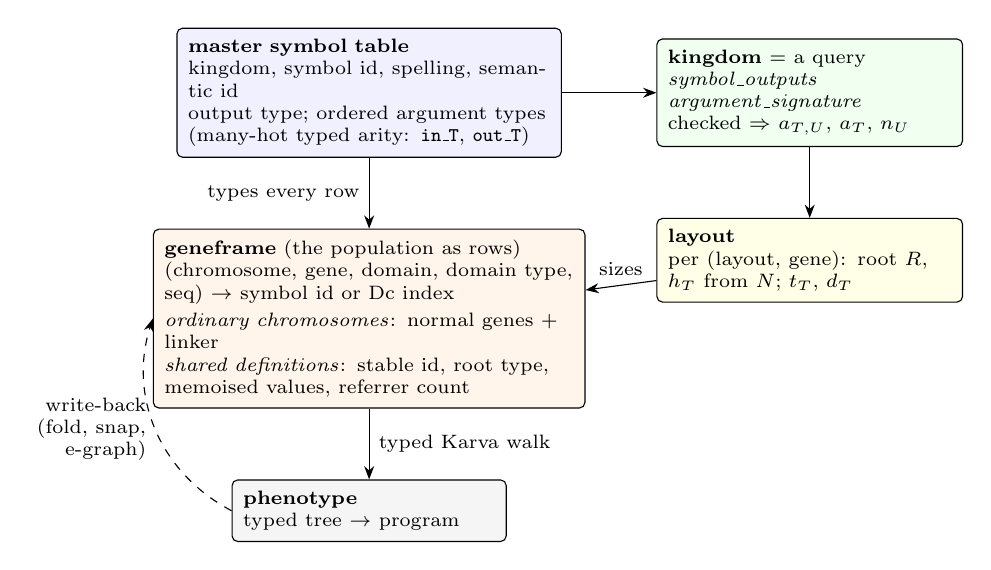
\begin{tikzpicture}[
  box/.style={draw,rounded corners=2pt,align=left,font=\scriptsize,inner sep=4pt,text width=#1},
  box/.default=4.2cm,
  hd/.style={font=\scriptsize\bfseries},
  >=Stealth]
\node[box=4.6cm,fill=blue!6] (tab) {\textbf{master symbol table}\\
kingdom, symbol id, spelling, semantic id\\
output type; ordered argument types\\
(many-hot typed arity: \texttt{in\_T}, \texttt{out\_T})};
\node[box=3.6cm,fill=green!6,right=1.2cm of tab] (k) {\textbf{kingdom} = a query\\
$\mathit{symbol\_outputs}$\\ $\mathit{argument\_signature}$\\
checked $\Rightarrow$ $a_{T,U}$, $a_T$, $n_U$};
\node[box=3.6cm,fill=yellow!10,below=0.9cm of k] (lay) {\textbf{layout}\\
per (layout, gene): root $R$,\\ $h_T$ from $N$; $t_T$, $d_T$};
\node[box=5.2cm,fill=orange!8,below=0.9cm of tab] (gf) {\textbf{geneframe} (the population as rows)\\
(chromosome, gene, domain, domain type, seq) $\to$ symbol id or Dc index\\[2pt]
\emph{ordinary chromosomes}: normal genes + linker\\
\emph{shared definitions}: stable id, root type,\\ memoised values, referrer count};
\node[box=3.2cm,fill=gray!8,below=0.9cm of gf] (ph) {\textbf{phenotype}\\ typed tree $\to$ program};
\draw[->] (tab) -- (k);
\draw[->] (k) -- (lay);
\draw[->] (lay) -- node[above,font=\scriptsize]{sizes} (gf);
\draw[->] (tab) -- node[left,font=\scriptsize]{types every row} (gf);
\draw[->] (gf) -- node[right,font=\scriptsize]{typed Karva walk} (ph);
\draw[->,dashed] (ph.west) to[bend left=40] node[left,font=\scriptsize,align=right]{write-back\\(fold, snap,\\e-graph)} (gf.west);
\end{tikzpicture}
\caption{The data model. The master symbol table types every row; a kingdom is a
query over it, checked into a contract; a layout derives the domain lengths; the
geneframe holds the population; the walk expresses it and the write-back encodes
rewrites back into it.}
\label{fig:geneframe}
\end{figure}

\section{Two row kinds: chromosomes and shared definitions}
Andrew's design of 2026-10-09 (\src{fuller/docs/PLAN_population_dag.md}, section 1)
gives the geneframe two row kinds: ordinary chromosomes, and population-wide
shared definitions. A shared definition is a gene tree with a stable row id, a
root type (so a reference to it is typed like a terminal of that type), memoised
row values and a count of referrers. An ordinary gene refers to it by a stable
id, never by a position. Folding is a variation operator: it adds definitions,
rewrites ordinary rows to refer to them, and re-sorts the definitions by use;
evaluation follows a level schedule in which a definition comes after everything
it references. The design's contract is determinism: values must be bit
identical with the shared rows present or stripped. The population is then its
own cache, with no kingdom-specific one.

The 2026-10-09 documents call these rows \emph{homeotic}. The code now follows
Ferreira's naming~\cite{ferreira2006adf}: the population-wide definitions are
ADFs, and \emph{homeotic gene} is reserved for a chromosome's typed linker
(\src{fuller/src/typed_chromosome.rs:1-25}). A homeotic gene has the per-type
layout of a normal gene; its alphabet is the whole epoch alphabet plus typed
genic terminals $G_g$, one for each normal gene it links; a fixed linker is a
homeotic gene marked immutable, and several homeotic genes form a multicellular
system with several main programs. ADF references $A_d$ are terminals of the
ADF's root type, and an ADF body may reference only ADFs of strictly lower
level; a genic terminal in a body is a defect (\src{:23}, \src{:84-106}). This
gives acyclicity by construction. The population DAG uses the same name for its
shared rows (\texttt{is\_adf}, \src{fuller/src/population_dag.rs:87}).

\paragraph{What is built.} The host side is built and tested: the epoch alphabet
with genic and ADF terminals (\texttt{Epoch::new},
\src{fuller/src/typed_chromosome.rs:162}), fixed and evolved linkers, ADF sets
(\src{:347}), fold by structural equality through the write-back
(\texttt{fold\_adf}, \src{:675}), unfold (\src{:383}), and a test that fold,
write-back and unfold preserve the value on random chromosomes (\src{:1074}). The population DAG --- hash-consed nodes, ADF rows,
memos keyed by node, data version, type and input binding, and the level
schedule --- is built on the host (\src{fuller/src/population_dag.rs}). The
device arena that would hold shared definitions on the GPU is not built
(\src{phylu/src/evolve/resident.rs:18-28}). Section~\ref{sec:eval-dag} gives the
measurements that decided this.

%======================================================================
\chapter{The GPU Implementation}
\label{ch:gpu}

phylu's typed core is a set of WGSL compute kernels driven through wgpu, with a
Rust host twin for every kernel. The twins are references for tests; the doc
comments of the twins state that they are not a search path
(for example \src{phylu/src/evolve/typed_init.rs}, \texttt{init\_row}).

\section{The device layout}
\texttt{typed\_layout.rs} turns fuller's \texttt{GeneLayout} into a device frame
table of ten words a frame --- type code, head offset and length, tail offset and
length, Dc offset and length, pool id, pool length and flags
(\src{phylu/src/evolve/typed_layout.rs:26}, packed at \src{:234}). The layout is
built on the host once, from the kingdom contract, and uploaded; it does not
change during a run. The population is held in a genome store that can be paged
across buffers (test {\small\path{a_paged_population_round_trips_through_the_device}},
\src{phylu/src/evolve/typed_layout.rs:557}).

\paragraph{Shader text independent of the layout.} The walk, initialisation,
variation and decode kernels are compiled from the shipped text with nothing
prepended, which a test asserts (\src{phylu/src/evolve/typed_walk.rs:616}); no
constant or array in them is derived from a layout. Per-invocation scratch is a
slice of a storage buffer, capacities are uniform fields, and a dispatch covers
as many whole rows as fit 256~MB of scratch
(\src{phylu/src/evolve/typed_decode.rs:425}, \src{phylu/src/evolve/typed_vary.rs:926}).
Two host contracts are checked from naga's reflection of the shipped text: no
kernel binds more than 29 buffers, Metal's limit for a stage, and each uniform
the host fills has the size of the struct the kernel reads
(\src{phylu/src/evolve/kernel_contracts.rs:1-13}). A layout of any width
therefore needs no change to a kernel.

\section{The kernels of one generation}
Table~\ref{tab:kernels} lists the typed core's kernels with their entry points.

\begin{table}[t]
\centering\small
\caption{The typed core's device kernels (phylu, \protect\src{src/evolve/}).}
\label{tab:kernels}
\begin{tabularx}{\textwidth}{@{}lYl@{}}
\toprule
stage & kernel entry points & host driver\\
\midrule
initialisation & \texttt{typed\_init\_main} (\src{typed_init.wgsl:100}); wrapper draw \texttt{typed\_wrapper\_main} (\src{typed_wrapper.wgsl:22}) & \src{typed_device.rs:468}, \src{:507}\\
expression (walk) & \texttt{walk\_main} (\src{walk_main.wgsl:51}) & \src{typed_walk.rs:250}\\
decode & \texttt{typed\_validate\_init\_main}, \texttt{typed\_validate\_main}, \texttt{typed\_decode\_main} (\src{typed_decode.wgsl:102}, \src{:112}, \src{:310}) & \src{typed_device.rs:870}\\
mutation & clone, point, leaf, mutate, gene transposition, Dc point, Dc mutate, RNC, cleanse (\src{typed_vary.wgsl:394}, \src{:419}, \src{:478}, \src{:541}, \src{:635}, \src{:664}, \src{:705}, \src{:748}, \src{:982}) & \src{typed_device.rs:600}\\
crossover & plan and swap passes (\src{typed_vary.wgsl:1049}, \src{:1095}) & \src{typed_device.rs:600}\\
selection & elite (parallel minimum), first, tournament, attributes (\src{typed_select.wgsl:231}, \src{:282}, \src{:294}, \src{:358}) & \src{typed_device.rs:600}\\
deduplication & \src{dedup.wgsl:67-256} & \src{dedup.rs}\\
\bottomrule
\end{tabularx}
\end{table}

\paragraph{Initialisation.} The initialiser draws each head by simulating the
walk queue, fills tail cells with terminals of their type and Dc cells with an
index below $|C_T|$; nothing is repaired afterwards. Device and host agree
bit for bit (tests {\small\path{device_init_equals_the_host_reference_on_{sr,regex,two_type}}},
\src{phylu/src/evolve/typed_init.rs:429-439}).

\paragraph{Expression and decode.} The walk kernel performs the typed Karva walk
of Chapter~\ref{ch:schema}; the decode kernel lays the expressed tree out as a
level-order node array for the evaluators and applies the kingdom's derived
attributes (for SR, transcendental depth). The host reference is fuller's
\texttt{express}, described in its own header as ``the test reference the GPU
decoder must match bit for bit, not a search path''
(\src{fuller/src/typed_gep.rs:20-21}); the tests are
{\small\path{the_walk_reference_equals_fullers_express}}
(\src{phylu/src/evolve/typed_walk.rs:521}) and
{\small\path{device_decode_equals_the_reference_*}}
(\src{phylu/src/evolve/typed_decode.rs:799-827}).

\paragraph{Variation.} \texttt{TypedDevice::vary} runs tournaments, attribute
gathering, mutation and recombination in one submission
(\src{phylu/src/evolve/typed_device.rs:600}). Crossover is two passes: a plan pass,
one thread per row, writes six words per pair; a swap pass, one thread per cell,
exchanges a cell exactly when an odd number of the three planned ranges covers it
(\src{phylu/src/evolve/typed_vary.wgsl:1040-1047}).

\paragraph{Selection.} The elite kernel is a parallel minimum; tournaments read
only the fitness buffer. The host twin \texttt{typed\_select\_twin.rs} must pick
the same rows, ties included (tests at \src{phylu/src/evolve/typed_device.rs:961},
\src{:1019}, \src{:1077}, the first comparing device and host over two whole
generations).

\section{The fitness contract}
Selection on the device reads one \texttt{f32} per individual from the
population's fitness buffer: an angle, zero perfect, lower fitter, as HFF
returns it. Variation copies an elite's fitness with the elite and marks every
new row NaN; the fitness evaluation fills exactly the NaN rows
(\src{phylu/src/evolve/resident.rs:13-14}, \src{:82-95}). Any kingdom that writes
this buffer --- from a device kernel or from the host --- is selected by the same
kernels. That is the whole interface between a kingdom's fitness and the
evolutionary core.

\section{The resident fitness chain}
For SR and regular expressions the fitness evaluation also runs on the device,
on one command buffer (\src{phylu/src/evolve/resident.rs:1-16}):
\texttt{decode\_main} $\to$ the evaluator over the resident node arrays $\to$
\texttt{score\_main} $\to$ \texttt{type\_main} $\to$ \texttt{colmax\_main}
(generation 0) $\to$ \texttt{hff\_main}, which writes the selection angle into the
population's fitness buffer where a row's fitness is NaN, that is, where the row
is new. One generation is brought back in one wait as a \texttt{Frame}: wrapper
ids, the fitness before HFF wrote it, the decoder's flags and depths, a per-gene
hash, and the winner records, ``a few kilobytes''
(\src{phylu/src/evolve/resident.rs:82-101}). The genes stay on the device; the
host reads individual rows when it acts on them (\texttt{read\_rows},
\src{phylu/src/evolve/typed_device.rs:593}; \texttt{hydrate},
\src{phylu/src/evolve/engine.rs:4685-4693}).

Figure~\ref{fig:dataflow} draws the two shapes the generation takes.

\begin{figure}[t]
\centering
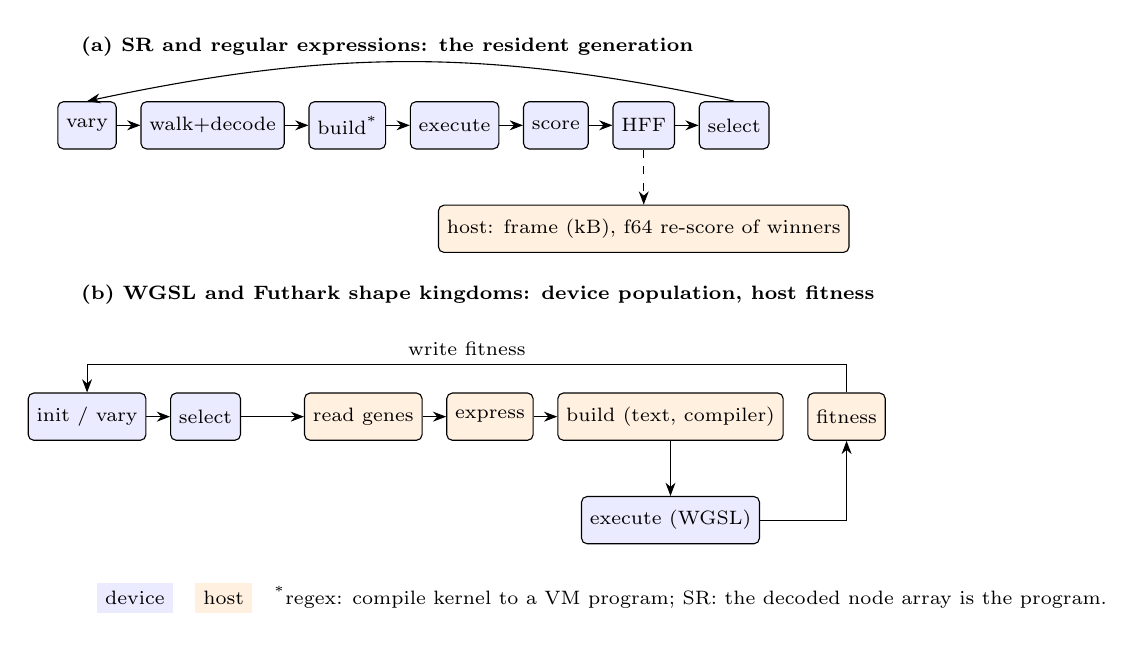
\begin{tikzpicture}[
  k/.style={draw,rounded corners=2pt,font=\scriptsize,minimum height=6mm,inner sep=3pt,fill=blue!8},
  h/.style={draw,rounded corners=2pt,font=\scriptsize,minimum height=6mm,inner sep=3pt,fill=orange!12},
  >=Stealth, node distance=3mm]
% Top: resident (SR, regex)
\node[font=\scriptsize\bfseries,anchor=west] at (-0.2,1.0) {(a) SR and regular expressions: the resident generation};
\node[k] (a1) at (0,0) {vary};
\node[k,right=of a1] (a2) {walk+decode};
\node[k,right=of a2] (a3) {build\textsuperscript{*}};
\node[k,right=of a3] (a4) {execute};
\node[k,right=of a4] (a5) {score};
\node[k,right=of a5] (a6) {HFF};
\node[k,right=of a6] (a7) {select};
\foreach \x/\y in {a1/a2,a2/a3,a3/a4,a4/a5,a5/a6,a6/a7} \draw[->] (\x) -- (\y);
\draw[->] (a7.north) to[bend right=12] (a1.north);
\node[h,below=7mm of a6] (r1) {host: frame (kB), f64 re-score of winners};
\draw[->,dashed] (a6.south) -- (r1.north);
% Bottom: WGSL and Futhark
\node[font=\scriptsize\bfseries,anchor=west] at (-0.2,-2.15) {(b) WGSL and Futhark shape kingdoms: device population, host fitness};
\node[k] (b1) at (0,-3.7) {init / vary};
\node[k,right=of b1] (b2) {select};
\node[h,right=8mm of b2] (b3) {read genes};
\node[h,right=of b3] (b4) {express};
\node[h,right=of b4] (b5) {build (text, compiler)};
\node[k,below=7mm of b5] (b6) {execute (WGSL)};
\node[h,right=of b5] (b7) {fitness};
\draw[->] (b1) -- (b2);
\draw[->] (b2) -- (b3);
\draw[->] (b3) -- (b4);
\draw[->] (b4) -- (b5);
\draw[->] (b5) -- (b6);
\draw[->] (b6) -| (b7);
\draw[->] (b7.north) -- ++(0,0.35) -| node[pos=0.25,above,font=\scriptsize]{write fitness} (b1.north);
\node[font=\scriptsize,anchor=west] at (0,-6.0) {\colorbox{blue!8}{device}\quad \colorbox{orange!12}{host}\quad
\textsuperscript{*}regex: compile kernel to a VM program; SR: the decoded node array is the program.};
\end{tikzpicture}
\caption{The two shapes of a generation. In (a) the host receives a frame of a
few kilobytes and acts on chosen rows. In (b) the genes cross to the host every
generation, the program is built there, and the fitness crosses back. In the
WGSL kingdom the kernel executes on the device; in the Futhark shape kingdom's
GPU-population runner it is interpreted on the host.}
\label{fig:dataflow}
\end{figure}

\section{External fitness}
For a kingdom whose fitness is evaluated on the host, the engine reads the whole
generation, scores the new rows and writes the fitness back
(\texttt{evaluate\_external}, \src{phylu/src/evolve/engine.rs:4645-4655};
\texttt{write\_fitness}, \src{phylu/src/evolve/typed_device.rs:557}). Selection
on the device then reads that buffer as it reads HFF's. This is the seam through
which the WGSL and Futhark kingdoms join the typed core.

\section{Checkpoints}
A resumed run must equal an uninterrupted one, so a checkpoint holds
everything the generation loop mutates: the genome, the constant pools $C_T$
(append-only, so every Dc index keeps its meaning), wrapper ids, fitness, cohort
labels and the band of rows the last immigration filled, with the seed and layout
checked on resume (\src{phylu/src/evolve/checkpoint.rs:51-100}, format version 3).
The JSON reader is built with exact floating-point round trips
(\texttt{serde\_json} feature \texttt{float\_roundtrip}, \src{phylu/Cargo.toml:37}),
because selection compares fitness values exactly.

%======================================================================
\chapter{The Kingdoms}
\label{ch:kingdoms}

Four kingdoms run on the typed core. Each section below gives the kingdom's type
system and where its generation runs; the search problems, the results and the
kingdom-specific machinery are the subject of the domain papers of this set,
cited in each section.

\section{Symbolic regression}
The untyped SR kingdom has one type, \ty{F}, over fuller's real-domain
\texttt{Math} operators (\texttt{master\_pset}, \src{fuller/src/karva.rs:59};
\texttt{master\_table}, \src{fuller/src/geneframe.rs:353}); its layout is
classical Karva. Andrew's typed SR (TSR) adds the depth types \ty{T1} and \ty{T2}
(\texttt{typed\_depth\_table}, \src{fuller/src/geneframe.rs:453-515}): terminals
are \ty{F}; arithmetic absorbs, returning the highest depth among its arguments;
a transcendental raises the depth by one; and no row accepts \ty{T2} as the
argument of a transcendental. The missing row is the rule: a model with three
nested transcendentals cannot be expressed. The rule follows a measurement of
the 133 SRBench ground-truth models, none of which nests transcendentals beyond
depth 2 (\src{fuller/src/geneframe.rs:468-470}). Later TSR variants generate
their types from tables (\texttt{Ty::Tsr}, \src{phylu/src/evolve/tsr_typed.rs}).
The program is the decoded node array, evaluated on the device by
\texttt{eval\_main} (\src{fuller/src/gpu_eval.rs:495}) and scored by
\texttt{score\_main} (\src{phylu/src/evolve/score.wgsl:276}). The whole generation
is device-resident. Domain paper:~\cite{tr_sr}.

\section{Regular expressions}
Four types: \ty{Pattern} (the root), \ty{CharClass}, \ty{Char} and the integer
\ty{I} for repetition counts (\src{fuller/src/regex_typed.rs};
\texttt{regex\_rows}, \src{fuller/src/geneframe.rs:521-561}). The types carry a
class algebra: ranges, negation and union build \ty{CharClass} values; coercions
lift a \ty{Char} or a \ty{CharClass} to a \ty{Pattern}; concatenation,
alternation, star, plus and option combine \ty{Pattern}s; counted repetition
\texttt{rep\_n(CharClass, I)} takes an integer count. The phenotype is compiled on
the device to a Thompson/Pike virtual-machine
program~\cite{thompson1968regex,cox2009regexvm} (\src{phylu/src/evolve/regex_emit.wgsl:49},
\src{phylu/src/evolve/regex_compile.wgsl:179}), executed over every labelled
value (\src{phylu/src/evolve/regex_match.wgsl:145}) and scored
(\src{phylu/src/evolve/regex_score.wgsl:75}) into the score row HFF reads
(\src{phylu/src/evolve/regex_resident.rs:1-10}). The whole generation is
device-resident. Domain paper:~\cite{tr_regex}.

\section{WGSL compute kernels}
\label{sec:wgsl}
The true WGSL kingdom is generated per interface by
{\small\path{kingdoms/wgsl_true/gen_tables.py}}; the instance committed beside the
generator has 305 types and 8,841 rows (\texttt{types.tsv},
\texttt{functions.tsv}). Each legality rule of WGSL is carried by a type
(\src{fuller/kingdoms/wgsl_true/README.md}): ownership types so that no two
threads write one element; statement types for uniform, conditional, write-phase
and epilogue contexts, so that barriers occur only in uniform control; bounded
loop types with capped trip counts and fuel strata, so that every loop ends;
index types, so that every index is in range; and rows whose spellings have only
WGSL-defined results. In-range index types \ty{u32.in\_<B>} (an index below
\texttt{arrayLength(\&B)}) remove the clamp from an access; they and a
compiler-assigned scatter, in which a gene names the cluster a value belongs to
and never a slot, are built for the k-means interfaces only
(\src{fuller/docs/DESIGN_inrange_index_types.md}). The device draws, varies and
selects the population; the host expresses, renders, compiles and scores each
kernel, which runs on the device (Chapter~\ref{ch:exec}). Domain
paper:~\cite{tr_wgsl}.

\section{Futhark array programs}
\label{sec:futhark}
In the shape kingdom (\texttt{kingdoms/futhark/}) a shape class is a type:
\ty{mat.n.m} is the interface's $[n][m]$ over three dimension roles, with nine
matrix classes and two function classes (a row function $[]f32\to[]f32$, and a
binary one, because Futhark's \texttt{map2} is curried): 11 types and 71 rows
(\src{fuller/kingdoms/futhark/types.tsv}, \texttt{functions.tsv}). The
unification of shapes is done once, offline, by the table generator, whose
witness tests re-check every shape relation, and a Rust test compares the
committed tables with what the generator would write; the engine sees an
ordinary typed kingdom. The \texttt{sig/} family holds one kingdom per published
benchmark (histogram, pathfinder, reduce, scan); the \texttt{pixel/} family holds
per-pixel programs in which scope, \texttt{let} and bounded loops are types. The
earlier 1-D kingdom (\texttt{kingdoms/futhark\_1d/}, 4 types, 38 rows) is
superseded. Two runners exist: phylu's \texttt{shape\_typed}, with the population
on the device and the evaluation in a host interpreter, and fuller's
\texttt{futhark\_evolve}, which compiles each program with the project's Futhark
fork (\texttt{rust-wgpu} backend, then \texttt{rustc}) and runs it on the device,
with a host genetic algorithm (Chapter~\ref{ch:exec}). Domain
paper:~\cite{tr_futhark}.

%======================================================================
\chapter{Execution and Fitness on the GPU}
\label{ch:exec}

This chapter states, kingdom by kingdom, where the program is built and
executed and where its fitness is evaluated. Table~\ref{tab:where} collects it.

\begin{table}[p]
\centering\small
\caption{Where each stage runs. \D{} device, \Hh{} host. ``Shape (GPU pop.)'' is
phylu's \texttt{shape\_typed} runner; ``Futhark sig'' is fuller's
\texttt{examples/futhark\_evolve.rs}. The layout is built on the host once and
uploaded in every kingdom.}
\label{tab:where}
\footnotesize\begin{tabularx}{\textwidth}{@{}>{\raggedright\arraybackslash}p{2.2cm}*{5}{Y}@{}}
\toprule
stage & SR / TSR & regex & WGSL true & Shape (GPU pop.) & Futhark sig\\
\midrule
gene layout        & \Hh{} once & \Hh{} once & \Hh{} once & \Hh{} once & \Hh\\
random genes       & \D & \D & \D & \D & \Hh\\
expression (walk)  & \D & \D & \Hh{} & \Hh{}\,(+\D{} walk check) & \Hh\\
variation          & \D & \D & \D & \D & \Hh\\
program building   & \D{} (node array) & \D{} (VM compile) & \Hh{} (render, naga, pipeline) & \Hh{} (interpreter; compiler for elites) & \Hh{} (fork compiler, rustc)\\
program execution  & \D & \D & \D & \Hh{} (interpreter) & \D\\
fitness evaluation & \D{} (f32), \Hh{} f64 confirm & \D & \Hh & \Hh & \Hh\\
selection          & \D & \D & \D{} (host fitness) & \D{} (host fitness) & \Hh\\
\bottomrule
\end{tabularx}

\medskip
\begin{tabularx}{\textwidth}{@{}lY@{}}
\toprule
cell & evidence\\
\midrule
SR, regex: all \D & \src{phylu/src/evolve/resident.rs:1-16}, \src{:82-101}; \src{typed_init.wgsl:100}; \src{typed_vary.wgsl:394-1095}; \src{typed_select.wgsl:231-358}; \src{fuller/src/gpu_eval.rs:495}; \src{score.wgsl:276}; \src{hff.wgsl:128}; \src{regex_compile.wgsl:179}; \src{regex_match.wgsl:145}; \src{regex_score.wgsl:75}\\
SR f64 confirm & \src{phylu/src/evolve/hff.wgsl:15-17}\\
WGSL init, vary, select \D & \src{phylu/src/evolve/true_wgsl_fit.rs:1-7}, \src{:771}, \src{:1445}\\
WGSL express, render \Hh & \src{phylu/src/evolve/true_wgsl_fit.rs:1736-1750} (\texttt{score\_row})\\
WGSL naga, pipeline \Hh; execute \D & \src{phylu/examples/wgsl_true_fit.rs:178-202}; \src{fuller/src/wgsl/harness.rs:3366}, \src{:3524}\\
WGSL fitness \Hh, written to \D & \src{phylu/examples/wgsl_true_fit.rs:210-219}; \src{phylu/src/evolve/true_wgsl_fit.rs:1308}\\
Shape: split as stated & \src{phylu/src/evolve/shape_typed.rs:10-27}; read genes \src{:425}; fitness written \src{:488}; walk check \src{:566}\\
Shape fitness & \src{fuller/src/futhark_search.rs:1091-1106} (\texttt{two\_level}, \texttt{fitness\_of})\\
Futhark sig: host GA & \src{fuller/examples/futhark_evolve.rs:790} (random gene), \src{:838} (mutation), \src{:867} (crossover); fuller cannot depend on phylu\\
Futhark sig: execute \D & \src{fuller/src/futhark_rust.rs:1-12}, \src{:274}\\
\bottomrule
\end{tabularx}
\end{table}

\section{Symbolic regression and regular expressions}
For both kingdoms the program is built on the device: in SR the decoded node
array is evaluated directly; in regex a compile kernel lowers the tree to VM
instructions. Execution and fitness evaluation are kernels on the same command
buffer as the decoder, and HFF writes the selection angle into the fitness
buffer that the selection kernel reads. The design claim that the generation
stays on the GPU is true for these two kingdoms, with three qualifications:
the host reads back a frame of a few kilobytes per generation; the winner is
re-scored in \texttt{f64} on the host before it is reported or stops a run; and
the operators outside the typed core --- constant snapping, the e-graph's
variants, and SRBench's symbolic check, which runs in Python --- are host work on
chosen rows (\texttt{snap\_winners}, \texttt{fold\_winners},
\src{phylu/src/evolve/engine.rs:5671}, \src{:6632}).

The reason for putting HFF on the device is recorded in the kernel: at a
population of 200,000 the host's HFF took 238~s of a 450~s fit, against 1.49~s
of GPU work (\src{phylu/src/evolve/hff.wgsl:1-7}).

\section{WGSL kernels}
The device initialises, varies and selects the population
(\src{phylu/src/evolve/true_wgsl_fit.rs:1-7}). Each generation the host reads
the genes, expresses each with fuller's \texttt{express}, inlines shared
definitions, renders the text and memoises it by text
(\src{phylu/src/evolve/true_wgsl_fit.rs:1736-1750}). naga parses and validates
the text; the runner also rejects, as an error that stops the run, a Metal
translation that carries the loop form Apple's compiler hangs on
(\src{phylu/examples/wgsl_true_fit.rs:178-188}). wgpu builds the pipeline, the
kernel runs on the device under a work bound (a submit over 1,000~ms of compute
stops the run, \src{:203-205}), and the host compares the output with the
reference on the cases and combines closeness and speed by HFF
(\src{:210-219}). The fitness is written to the device for selection
(\src{phylu/src/evolve/true_wgsl_fit.rs:1308}).

So in this kingdom the GPU runs the population and the evolved programs, but the
programs are built on the host, and the fitness is computed on the host and
returned to the device. Building on the host is not incidental: the shader
compiler (naga, then the platform's compiler) is host software. Two parts could
move: expression, since the walk kernel exists and is already used for checking
in the shape kingdom; and the comparison of outputs, for which the harness has a
device judge (\texttt{pooled\_judge.wgsl}, \src{fuller/src/wgsl/harness.rs:3442}).
Neither is wired into the true-kingdom runner today.

\section{Futhark programs}
\paragraph{The shape kingdom with a GPU population.} The runner's header states
the split, and the code follows it (\src{phylu/src/evolve/shape_typed.rs:10-27}).
The device draws, varies and selects the population and walks each gene; the
walk's node count is compared with the host's expression
(\texttt{walk\_check}, \src{:566}). The host reads the generation (\src{:425}),
expresses each gene, interprets it with the shape kingdom's interpreter, and
computes the static cost. The fitness is the two-level HFF: TrueNorth over the
quality group (disagreement with the reference on each input set, on HFF's log
scale), then over the speed group (traffic, allocations and serial depth, each
as $x/(x+x_{\mathrm{ref}})$), then over the two angles
(\src{fuller/src/futhark_search.rs:1084-1106}). It is written to the
device at \src{phylu/src/evolve/shape_typed.rs:488}. A gene that the layout cannot
express would score 1.5 (\src{:455}).

The reason the evaluation is on the host is stated in the runner and the
paper: the device's backend contracts multiply-add into FMA and the interpreter
does not, so on a matrix product 758 of 4,096 elements agreed bit for bit, and the
correctness contract is bit-exact (\src{phylu/src/evolve/shape_typed.rs:23-26};
\src{phylu/docs/paper/shape_typed_gecco_paper.tex}, section ``The GPU/Host Split'').
The ``measured GPU cost'' is obtained by compiling the program and parsing the
compiled GPU program, for the best correct individuals only.

\paragraph{The benchmark runner.} fuller's \texttt{futhark\_evolve} runs the
\texttt{sig/} kingdoms. Because fuller does not depend on phylu, this runner has
its own host genetic algorithm: random genes, point mutation, homologous
crossover and typed subtree crossover are host code over fuller's layout
(\src{fuller/examples/futhark_evolve.rs:10-22}, \src{:790}, \src{:838}, \src{:867}).
Candidates are compiled to WGSL through the fork's \texttt{rust-wgpu} backend and
\texttt{rustc}, and executed and timed on the device. The fitness is a staged HFF
computed on the host.

\paragraph{What would complete it.} For the shape kingdom, the evaluation moves
to the device only with a device evaluator that reproduces the interpreter's
arithmetic bit for bit (no FMA contraction, the same reduction order), or with a
change of the correctness contract; the compile, as in WGSL, is host software. For
the benchmark runner, moving its selection and variation onto phylu's typed core
through the external-fitness seam would give it the device population the other
kingdoms have.

%======================================================================
\chapter{GPU-Driven Evolution}
\label{ch:evo}

\section{The generation}
In every kingdom on the typed core, a generation is: selection and variation on
the device in one submission; fitness evaluation, on the device's resident chain
or through the external-fitness seam; and selection of the next generation's
parents from the fitness buffer. Elites keep their fitness by copy; new rows are
marked NaN and scored. Deduplication by gene hash is on the device.

\section{Operators outside the typed core}
Every operator outside plain GEP variation writes back through the typed codec, so
its children are feasible by the same argument as the core's. In SR these are
constant snapping and a near-constant collapse; in the Futhark and WGSL kingdoms,
the e-graph's equivalent forms of elites (a local search on the cost axis, since
its rules are equalities), a pump that injects the best individuals' variants, and
typed subtree crossover between parents with different expressed trees. All of
these run on the host on a few rows, and each emits a mutation event to the run's
telemetry stream (\src{fuller/CLAUDE.md}, ``Every evolution runner meets one
standard''; \src{phylu/docs/WATCHER.md}).

\section{Is it fully on the GPU?}
The claim ``GPU programs built on the GPU, executed on the GPU, with the fitness
returned on the GPU and directly driving GPU-based evolution'' holds as follows.
\begin{itemize}
\item \textbf{SR and regex: true.} The programs are built, executed and scored on
the device and the fitness drives the device's selection, with a kilobyte frame
and an \texttt{f64} confirmation on the host. These programs are expressions and
regular expressions evaluated by device interpreters, not GPU programs in their
own right.
\item \textbf{WGSL: partly.} The evolved programs are GPU programs and run on the
device, and the population, variation and selection are on the device. The
programs are built on the host (expression, rendering, naga, the driver's
compiler) and the fitness is computed on the host and uploaded.
\item \textbf{Futhark shape kingdom (GPU population): partly.} Population,
variation and selection are on the device; execution in the fitness evaluation
is the host interpreter, and compiled GPU programs are analysed only for elites.
\item \textbf{Futhark benchmark runner: execution only.} The programs run on the
device; the evolution is on the host.
\end{itemize}

%======================================================================
\chapter{Evaluation}
\label{ch:eval}

Every figure below is quoted from the file named with it. Each is one machine
(an Apple M3 Max laptop, wgpu over Metal) unless stated, and most are one or few
seeds. This chapter summarises what bears on the shared design; the full
evaluation of each kingdom is in its domain
paper~\cite{tr_sr,tr_regex,tr_wgsl,tr_futhark}.

\section{The rebuild onto the typed core}
\paragraph{SR non-regression.} Moving SR onto the typed core was checked by
running the old and new engines on 100 laws with ten seeds each: 481 of 1,000
seed-runs passed the stopping criterion on both
(\src{fuller/docs/reports/2026-10-20_multityped_gep_rebuild.md}, section 2.1). SR
is single-typed, so this tests non-regression only; the arms draw different
random numbers and no paired test was run.

\paragraph{Regular expressions.} On the UK-postcode task (198 unseen postcodes,
600 foreign-format and 200 corrupted-UK negatives, seeds 7013--7016), the typed
core reached 100.0\,\% held-out recall in every typed configuration against
97.5\,\% for the previous multi-typed engine, with no foreign format accepted in
either; corrupted UK values accepted fell from 104 of 200 to between 0 and 12.
The rules are longer (54 characters against 17), and the typed core evaluated far
fewer individuals in the same time: at equal budget it ran at 28--30\,\% of the
old generation rate (\src{fuller/docs/reports/2026-10-20_multityped_gep_rebuild.md},
sections 2.2 and 2.3). The plan's throughput expectation was missed. An earlier
comparison on the previous engine (one seed, 180~s) measured the four-type
kingdom against a single-type one at 97.5\,\% against 92.4\,\% held-out recall,
with corrupted-UK acceptance worse, 26 of 50 against 14
(\src{phylu/docs/reviews/2026-10-04_multityped_regex_result.md:42-54}).

\section{Symbolic regression on SRBench}
On the 133 SRBench ground-truth problems~\cite{lacava2021srbench}, one development
seed, 90~s a problem, the typed-depth engine recovered 74 laws by SRBench's own
symbolic check, and fuller's post-search candidate generation 5 more, 79 of 133
(\src{phylu/docs/TYPED_ENGINE.md:20-25}; \src{fuller/papers/geneframe-gecco.tex},
section ``Results as Highlights''). This was measured on 2026-09-30, on the engine
before revision 4, in which typing was applied by the decoder and ill-typed genes
were refused (31 million over the 133 runs). It is not SRBench's protocol, which
counts exact solutions over ten runs with a budget of hours; AI
Feynman~\cite{udrescu2020aifeynman} solves about 53\,\% of runs at zero noise under
that protocol. We report the count as one seed under a weaker protocol, not as a
comparison.

\section{Device throughput}
Before revision 4, on the device engine, a regex generation at population 2,600
took 10~ms multi-typed and 21~ms single-typed, and SR at population 2,000 took
46~ms (\src{fuller/papers/geneframe-gecco.tex}, Table ``throughput''). On the typed
core the regex generation was 11.9 to 16.5~ms at $N=28$ against 7.3~ms for the old
build (\src{fuller/docs/reports/2026-10-20_multityped_gep_rebuild.md}, section 2.3).
The layout-independent kernels keep scratch in device memory rather than private
memory, which the design notes expected to cost time.

\section{The WGSL kingdom}
\label{sec:eval-wgsl}
\paragraph{The k-means centroid update.} The task was a faster drop-in for
UltraDim's centroid update (A7, a gather, $O(knd)$). Generation 0 held A7, a
hand-written counting-sort ``scatter'' form ($O(nd)$) and A7's point mutants; the
run took 1,415 evaluations over 97 generations. At $n=8{,}192$, $d=256$,
$k=1{,}024$, in 11 interleaved pairs with A/A checks passed, the champion ran at
0.0273 of A7's time and 0.9840 of the hand-written scatter form's, faster in 11 of
11 pairs each, with outputs bit-identical to A7's on all 8 cases
(\src{fuller/docs/kmeans_champion_s1/README.md}). Almost all of the speed is the
algorithm, which was given, not found: ``Evolution did not invent the scatter. It
made the scatter form 1.6\,\% faster.'' The likely source of that 1.6\,\% is that
the champion's Kahan compensation reads a register that is never written, so the
sum is plain; this is bit-safe on Metal, whose compiler already removes A7's
compensation (8 of 8 cases,
\src{fuller/docs/reports/2026-10-28_metal_removes_a7_kahan.md}), and is not
measured on Vulkan.

\paragraph{The cost of the kingdom's spelling.} Rewritten into the kingdom's own
spelling, the hand-written scatter form ran at 1.0255 and 1.0238 of its original
text; the cause was the index clamp on every access
(\src{fuller/docs/papers/2026-10-31_kmeans_centroid_update.md}, section 2). After
the in-range index types and the compiler-assigned scatter, the segmented form as
expressed ran at 0.2319~ms in total against 0.2315~ms for the yardstick and
0.2318~ms as written (\src{fuller/docs/DESIGN_inrange_index_types.md}, section 10).

\paragraph{Earlier WGSL kingdoms.} Before the true kingdom, on the earlier
\texttt{safewgsl} kingdom, structural rules with selection made correct Gram
kernels 1.19$\times$ and 1.25$\times$ faster than generation 0's best (paired,
6 of 6), and evolution from random genes found no correct kernel in 180
generations (\src{fuller/docs/reports/2026-10-13_SUMMARY.md}). A homologous
section crossover produced correct children in 42 of 276 cases (15.2\,\%) against
19 of 284 (6.7\,\%) for typed Karva crossover, without a reliably faster best
kernel (\src{fuller/docs/reports/2026-10-15_nluca_per_width.md}). Section crossover
is not part of the typed core.

\section{The Futhark kingdoms}
\paragraph{A7 matrix kernel.} On the shape kingdom's A7 kernel (two matrix
products added) at $n=m=p=64$, the reference's OpenCL kernel is too large for the
device to compile (error $-48$); the search found a form that runs, with 9 device
allocations against 15 ($-40\,\%$), 106,496 bytes against 188,416, and 5 kernels
against 10; the static traffic fell from 45,056 to 20,480
(\src{fuller/docs/measurements/2026-10-27_futhark_shapes_A7.md}, lines 25--66). The win came from the e-graph's transposed-product rule
and Futhark's own common-subexpression elimination, and the winner is untiled
where the reference is tiled. The e-graph's rule fired in generation 0 and never
again. With the population in the device's typed core ($n=m=p=8$, 32
individuals, 20 generations), mean agreement rose from 0.031 to a peak of 0.375,
and the correct count oscillated between 5 and 12 of 32
(\src{phylu/docs/paper/shape_typed_gecco_paper.tex}, ``The GPU-resident
population'').

\paragraph{Published benchmarks.} On four benchmarks from
\texttt{diku-dk/futhark-benchmarks} with 1,400 evaluations a run, evolution and
random search both found the two-node reduce and scan exactly in 3 of 3 seeds,
random search slightly sooner, and neither found the 7-node histogram or the
24-node pathfinder (\src{fuller/docs/reports/2026-10-27_STUDY_evolving_benchmarks_summary.md}).
After the fitness was corrected (Section~\ref{sec:faults}), evolution with point
mutation reached a lower best HFF than random search in 4 of 4 pairs at equal
numbers of programs scored --- histogram 1.0584 against 1.1346 and 0.9513 against
1.0608, pathfinder 0.9834 and 0.9536 against 1.0000 --- and found no exact
program (\src{fuller/docs/reports/2026-10-29_futhark_reruns.md}). Two of the
histogram runs stopped at the 30-minute bound because of compile failures.

\section{The population DAG}
\label{sec:eval-dag}
On sixteen exported generation pairs of a real unsolved SR population
(\texttt{strogatz\_predprey1}), the shared DAG did 33.3\,\% of an interpreter's
operator evaluations, and 24.5\,\% with the previous generation's memos, with
values bit-identical, on the host (\src{fuller/docs/PLAN_population_dag.md},
section 2c). On the device the shared DAG was slower: 7.8~ms a generation against
6.4~ms for the interpreter (+23\,\%), because at 400 rows the evaluation is not
arithmetic-bound and the DAG adds 16 to 21 level passes; the host fold took 400~ms
(\src{fuller/docs/PLAN_population_dag.md}, section 2f). The DAG's device arena was
therefore not built.

%======================================================================
\chapter{Discussion: Faults Found and What They Taught}
\label{ch:discussion}
\label{sec:faults}

\paragraph{Refusal hides bugs and flattens the search.} Before revision 4 the
decoder typed genes at expression time and refused ill-typed ones, and a shared
head mixed types: 31 million genes were refused over the 133 SRBench runs, and on
one problem 7\,\% of decoded genes (\src{fuller/papers/geneframe-gecco.tex}). The
per-type layout and the exact bounds of revision 4 are the answer: nothing is
refused because nothing ill-typed can be expressed.

\paragraph{A bound must count producers, not types.} The advisor's review of
revision 3 found that its tail bound, $t_T=\min(H a_T+[T=R],\ldots)$ with
$H=\sum_T h_T$, grew with the square of the type count: about 8 million words a
gene for a 204-type WGSL kingdom (\src{fuller/docs/reviews/2026-10-20_multityped_gep_fable.md},
finding 1). Counting demand per producer (equation~\eqref{eq:tail}) removed it.
The same review found that genic terminals could escape their type when a gene's
root travelled with the record, and that a fixed-length gene cannot hold an
arbitrary folded subtree; the answers --- roots belong to the layout, ADFs are
stored as expressed trees --- are now in the code.

\paragraph{The device and the language disagree at the edges.} naga wrote
integer division and remainder to Metal unguarded, where WGSL defines $x\%0=0$;
about 140 of 1,000 random kernels carried one, and one hung the GPU after its
process died. Every integer division whose divisor may be zero is now written
guarded (\src{fuller/docs/reports/2026-10-13_SUMMARY.md}). The lesson for a typed
kingdom is that ``no undefined behaviour'' has to be a property of the rows'
spellings on every backend, not only of the language specification.

\paragraph{Measurements can reward the wrong program.} A $u32$ overflow in a
guard made a kernel do no work at the timing size and claim a 450$\times$ speed-up;
both kernels that used it were withdrawn, and every timed output is now checked
against the yardstick's. Fresh buffers per run moved one entry's speed by up to
25\,\%. 37 of 40 earlier random kernels raced, so earlier random searches were
partly selecting on race noise (\src{fuller/docs/papers/2026-10-31_kmeans_centroid_update.md},
section 3; \src{fuller/docs/reports/2026-10-13_SUMMARY.md}).

\paragraph{A fitness must order neighbours of the target.} In the first Futhark
benchmark study the fitness became worse as programs came closer to the target
(Spearman $-0.68$ on histogram, $-0.52$ on pathfinder), an all-zeros output
scored better than the median wrong non-zero output, and one-edit neighbours of
the target scored inside the plateau. A review listed 22 faults, six of which
broke evolution (\src{fuller/docs/PLAN_futhark_fitness_fixes.md}). After the
quality inputs were replaced and checked against the slope criterion, evolution
beat random search in 4 of 4 pairs. A remaining fault: in the two-level HFF,
wrong but fast mutants outranked an exact seed, so that run was stopped and a
correctness constraint was planned (\src{fuller/docs/reports/2026-10-29_futhark_reruns.md}).

\paragraph{Sharing that pays on the host need not pay on the device.} The
population DAG saves a factor of four in operator evaluations and costs 23\,\%
more device time at the SR shape, because one dispatch over 12,000 genes costs
about the same whatever they hold. The same measurement found genes whose values
differ between a single invocation and a stored intermediate on this platform's
fast-math transcendentals, which a shared evaluation would have to settle
(\src{fuller/docs/PLAN_population_dag.md}, section 2f).

\paragraph{The types pay where they carry a rule.} The in-range index types
removed the clamp cost on the k-means kernel; before them, the kingdom's spelling
made the hand-written scatter form 2.4 to 2.6\,\% slower. This is the design's
own check, ``does this step put the rule into the symbol table's types?''
(\src{fuller/docs/GOAL.md}), applied to a measured cost.

%======================================================================
\chapter{Limitations and Future Work}
\label{ch:limits}

\begin{itemize}
\item \textbf{Host stages in two kingdoms.} WGSL and Futhark build programs and
evaluate fitness on the host, and the genes cross to the host every generation.
Moving expression to the device kernel that exists, and the WGSL output
comparison to the device judge, would remove part of this; the compile remains
host software in both.
\item \textbf{A second Futhark runner.} The benchmark runner duplicates the
typed core's operators on the host. Running it on phylu's core through the
external-fitness seam would give it a device population.
\item \textbf{Results are few-seed and one machine.} The SR count is one seed under
a weaker protocol than SRBench's; the regex comparison has no external baseline;
the WGSL champion is one seed on Metal only; the Futhark A7 result is one kernel.
\item \textbf{Evolution has not found the hard targets.} No correct WGSL kernel from
random genes on the earlier kingdom; no exact histogram or pathfinder program; the
k-means algorithmic gain was supplied, not discovered.
\item \textbf{Throughput fell on the rebuild} for regex, to 28--30\,\% of the
previous generation rate.
\item \textbf{The ADF rename and the device arena} for shared definitions are not
done; the device measurement says the arena would not pay at the SR shape.
\item \textbf{The head draw} is not settled by measurement.
\end{itemize}

%======================================================================
\chapter{Conclusion}
\label{ch:conclusion}

Andrew Morgan's design gives GEP a head and a tail for every output type, with
head lengths $h_T=[T=R]+(N-1)\,a_T$ and exact per-producer tail bounds derived
from a kingdom's ordered signatures. It holds the language in a master symbol
table, a kingdom as a query over it, and the population as rows of the
geneframe. Validity is a property of the layout, so the same variation operators
serve every kingdom with no repair. The code bears this out: one typed core in
WGSL initialises, decodes, varies and selects populations of four kingdoms, with
a host twin and an equality test for every kernel.

The claim that the whole loop stays on the GPU is true for symbolic regression
and regular expressions, where programs are built, executed and scored on the
device and the fitness drives the device's selection. It is partly true for WGSL
kernels and Futhark programs: the population and its evolution are on the device
and the evolved WGSL kernels run there, but the programs are built and scored on
the host, for reasons of compiler software and of bit-exact correctness. The
measured results are modest and stated as such: non-regression for SR, a gain in
held-out recall for regular expressions at a cost in throughput, a 1.6\,\% gain
on a supplied k-means algorithm, a Futhark kernel that compiles where its
reference does not, and benchmarks on which evolution beat random search without
reaching the target.

\bibliographystyle{plainnat}
\bibliography{multityped_gep_gpu_core}

\end{document}
